\documentclass[a4paper,12pt]{article}
\usepackage{graphicx}
\usepackage{hyperref}
\usepackage{url}
\begin{document}
\title{Box2D Project Report \\  Group 21 \\ Vulcans! \bigskip}
\author{
  Anand Dhoot\\
  \texttt{130070009}
  \and
  Maulik Shah\\
  \texttt{13D100004}
  \and
  Anchit Gupta\\
  \texttt{13D100032}
}
\date{\today}
\maketitle

\pagebreak
\begin{section}{Introduction}
\label{sec:Intro}
A Rube-Goldberg machine is a deliberately over-engineered or overdone machine that performs a very simple task in a very complex fashion, usually including a chain reaction. We have designed once such contraption (imagined by us in the very First lab), which we (Finally) present here. We used Box2D, a 2-dimensional physics simulation engine (written in C++) to code/implement it. Firstly, in the report, we describe the intention and structure of our machine (and differences from the originally conceived idea).
\linebreak
\linebreak
Inspired by the festive season and our love for fireworks we decided to go with a festive theme. A very clever boy loves fireworks but is
afraid to light them and just likes to see them from a distance. So he builds a Rube Goldberg Machine to solve his problem.
After starting the machine and positioning the fireworks the boy gets enough time to go back a safe distance and climb on to the roof of his house to witness the show.
\end{section}
\bigskip
\pagebreak

\begin{section}{Contents}
\tableofcontents
\end{section}
\pagebreak

\begin{section}{Honor Code}
We pledge on our honour that we have not given or received any unauthorized assistance in this assignment or any previous task.
\end{section}
\bigskip

\begin{section}{Schematic}
Original schematic is as follows \\
\\
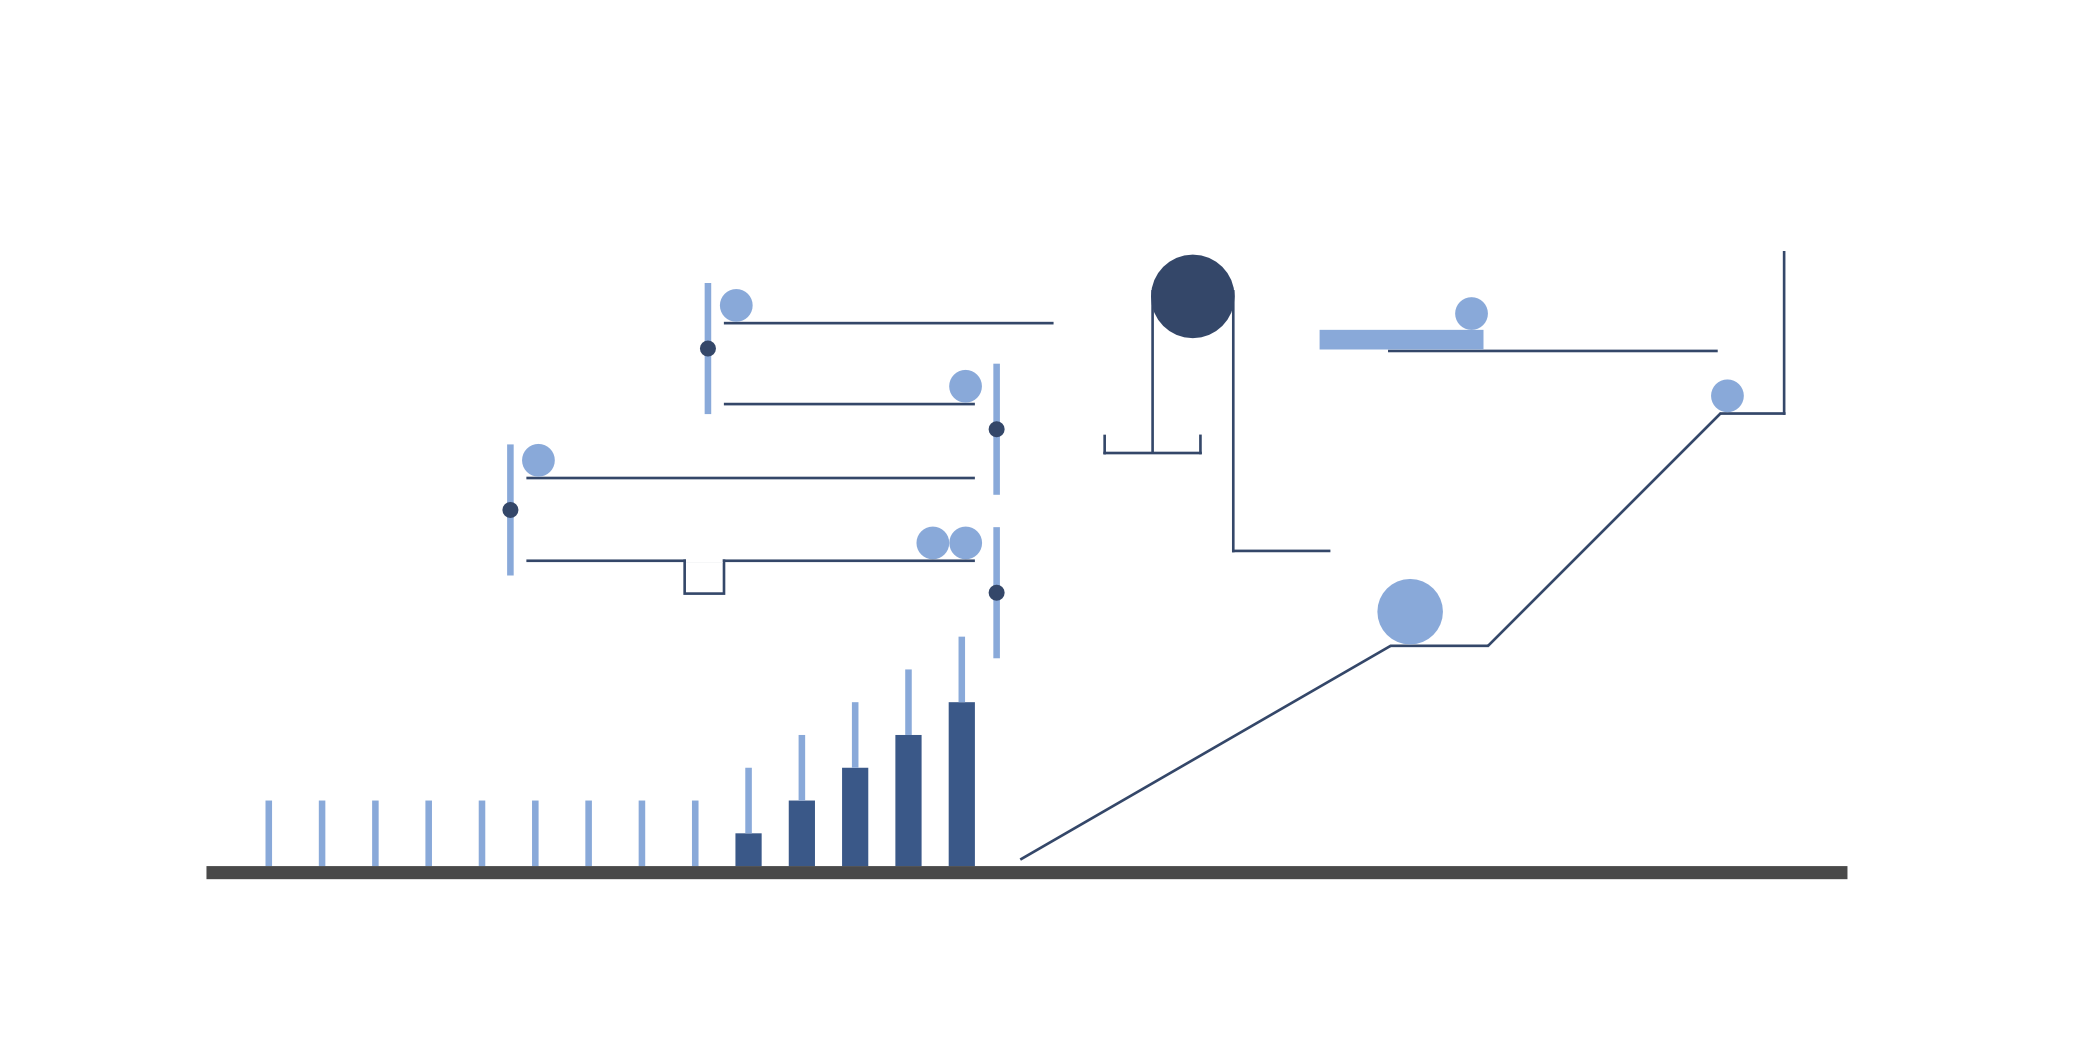
\includegraphics[scale=1.55]{./Images/rect3049.png}
\\
After considering various inputs that we got from our Instructor, TAs and the graders and given the fact that the course taught us new things which we decided to use, we added several new components to our original design.A screenshot of our final machine is - \\
\begin{center}
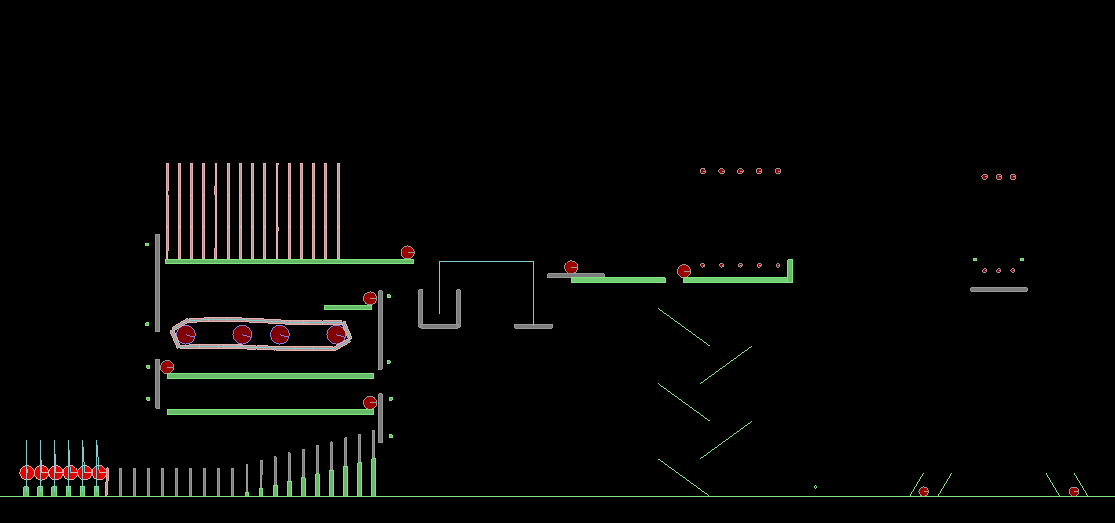
\includegraphics[scale=0.3]{./Images/FinalDesign.png}
\end{center}
\begin{subsection}{Differences Between old and new designs}
\begin{enumerate}
\item We replaced one of the horizontal levels by a conveyor belt. This was done so as to increase the complexity as well as improve the speed of the simulation.
\item The  top level of the shelves was replaced by a sequence of  vertically stacked dominoes this further improves the run time and is more aesthetically pleasing.
\item Fireworks - we decided to change the ending of our project and being inspired by the festive season we decided to put on a fireworks display as the grand ending.
\item Canons - to trigger the final cracker we added a few cannons which were triggered simultaneously and converged on final triggers for the ending.
\item Steps - We replaced the initially planned inclined plane by a series of steps to better redirect the potential energy of the ball.
\end{enumerate}
\end{subsection}
\end{section}
\bigskip

\begin{section}{Components Used and their physical aspects}
\begin{subsection}{Newton's Pendulum}
\begin{center}
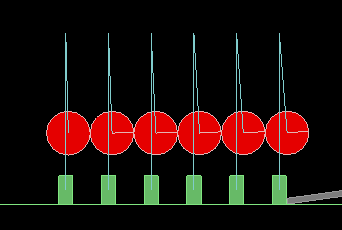
\includegraphics[scale=.45]{./Images/NewtonsPendulum.png}
\end {center}
The simulation is triggered by a Newton's Pendulum which is basically a set of adjacent simple pendulums which
beautifully demonstrate the principles of momentum conservation,energy conservation and impulses. \\
A simple pendulum is a weight suspended from a pivot so that it can swing freely about its equilibrium position. When released, the restoring force combined with the pendulum's mass causes it to oscillate about the equilibrium position, swinging back and forth. The differential equation which represents the motion of a simple pendulum is
$${d^2\theta\over dt^2}+{g\over \ell} \sin\theta=0$$
where \(g\) is acceleration due to gravity, \(\ell\) is the length of the pendulum, and \(\theta\) is the angular displacement.
\end{subsection}

\begin{subsection}{Dominos}
\begin{center}
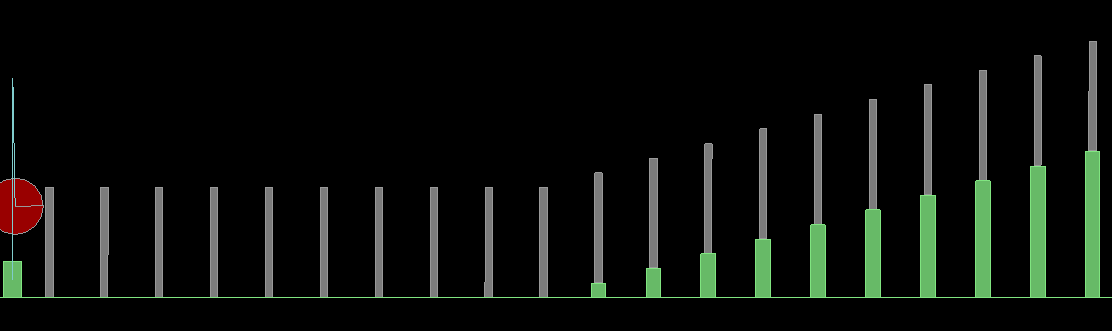
\includegraphics[scale=.25]{./Images/LowerDominos.png}
\end{center}
Dominoes have been used quite a bit in the simulation as means to quickly transfer momentum and thus keep the viewer engaged.
The simulation of dominoes is a very good way to demonstrate the capabilities of the Box2D Physics Engine and thus we used it.

Fall of the dominos can be interpreted to be caused by an impulse. Following is the equation that every domino would follow
$$ J*R = I*\alpha $$
where \(J\) is Impulse on the domino from the previous domino, \(R\) is height of domino, \(I\) is moment of inertia of the domino about point of contact with ground and \(\alpha\) is angular acceleration of domino.
\end{subsection}

\begin{subsection}{Balls}
In our simulation Balls have been extensively used as a medium to transfer energy from one part of the simulation to
the other.

The balls in the context of our theme represent pieces of flint stone which when rubbed with metal give rise to sparks to light the fireworks and the canons. Thus going with this theme we have changes the color of all the balls to red to represent their fire lighting capability.
\end{subsection}

\begin{subsection}{Conveyor Belt}
\begin{center}
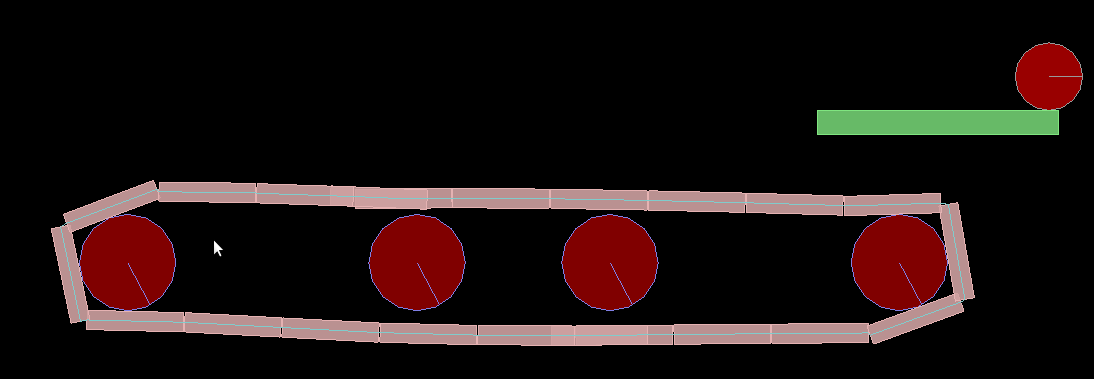
\includegraphics[scale=.25]{./Images/ConveyorBelt.png}
\end{center}
The conveyor belt in our design has been added to showcase yet another capability of Box2D - the ability to mechanise bodies. The conveyor belt in our design carries the ball from one side to another quickly.

The idea was implemented as a rectangular chain. Then, we add rotating discs in the chain. We keep a very high friction between these discs and the chain and give the discs a constant angular velocity, due to which the conveyor belt rotates
\end{subsection}

\begin{subsection}{Pulley}
\begin{center}
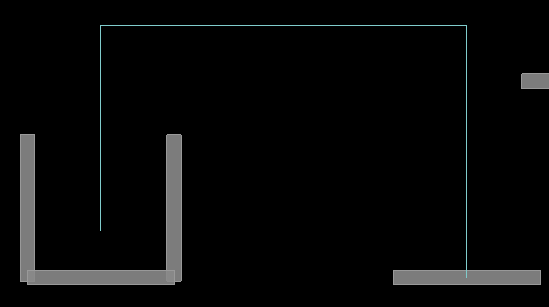
\includegraphics[scale=.35]{./Images/Pulley.png}
\end{center}
A pulley is a simple machine that is designed to support movement and change of direction of a cable or belt along its circumference. Pulleys are used in a variety of ways to lift loads, apply forces, and to transmit power.

In our project, we have used to pulley as an element of the Rube Goldberg machine to trigger the next set of events. When the ball falls into one side of the pulley, which causes the right side to move up. Essentially, this uses the force of gravity on the ball to push the plank on the right upwards for the next stage of the simulation.
\end{subsection}

\begin{subsection}{Explosions}
\begin{center}
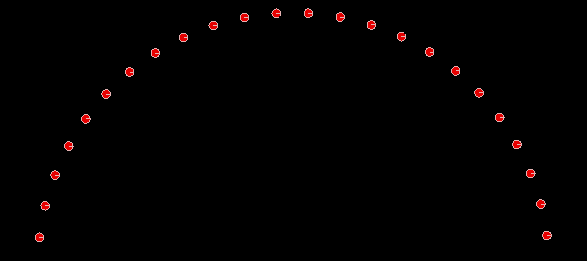
\includegraphics[scale=.33]{./Images/Explosion00.png}
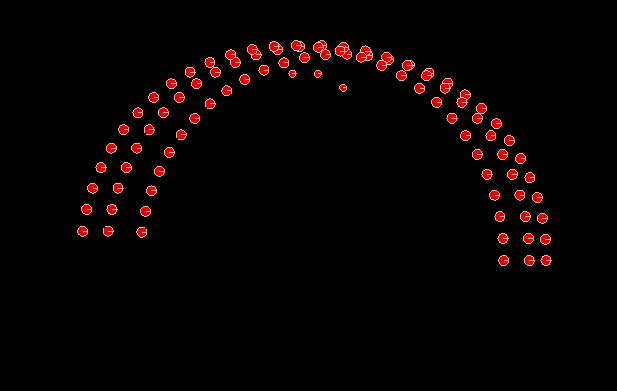
\includegraphics[scale=.22]{./Images/Explosion02.png}
\end{center}
This element is the centerpiece of our whole simulation. We have placed multiple triggers and fireworks all around the simulation
which are triggered at different times in the sim. Going with the theme of the festive season these explosion we think quite
realistically simulate the real deal and add an element of  novelty and uniqueness to our project.
\end{subsection}

\begin{subsection}{Canons}
\begin{center}
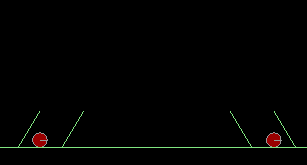
\includegraphics[scale=.35]{./Images/Cannon00.png}
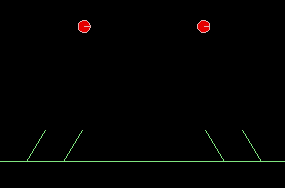
\includegraphics[scale=.35]{./Images/Cannon01.png}
\end{center}
This is also quite interesting the finale of our simulation is triggered by  two canons which launch a projectile.
Projectile motion is a form of motion in which an object or particle (called a projectile) is thrown near the earth's surface, and it moves along a curved path under the action of gravity only. The only force of significance that acts on the object is gravity, which acts downward to cause a downward acceleration.The trajectory followed by the object is a parabola and is described by  
$$y = xtan\alpha - \frac{1}{2}\frac{g x^2}{u^2 cos^2 \alpha}$$
The canons in our simulation shoot projectiles which follow this equation and using this we have a
carefully aligned them so as that they converge to a common point $\oplus$ and thus be able to provide enough force so as to push the plank which triggers the finale.
\end{subsection}
\end {section}
\bigskip

\begin{section}{Implementation Plan}
\begin{itemize}
\item
Phase 1: We started from the bottom up first implementing the bottom-most pendulums and the staggered dominoes.
\item
Phase 2: Added the horizontal platforms and the hinged joints.
\item
Phase 3: This phase involved constructing the conveyor belt and testing it. Subsequently we improved it to make the belt tighter wound on the rollers
\item
Phase 4: Integration of all elements mentioned above. This included fine-tuning the size and position of each element so that the entire sequence of events happens perfectly. Balls were added along with the top level of layered dominoes.
\item
Phase 5: Implemented the triggering mechanism, the Explosion class and the mycontactsolver class (to do explosions when the trigger is activated).
\item
Phase 6: The pulley and the right platforms were added and the top level of the explosion was integrated into the simulation.
\item
Phase 7: The step maze was added along with the cannons and the final flourish was implemented.
\item
Phase 8: Final integration of all elements for the perfect sequence of events. This involved extensive testing.
\item
Phase 9: Making the Executive Presentation, Documentation etc
\end{itemize}
\end{section}
\bigskip

\begin{section}{Task Distribution}
Most phases had inputs from all team members. Broadly, the task distribution was as follows -
\begin{enumerate}
\item Anand Dhoot - Phases 4, 6 and 7
\item Maulik Shah - Phases 1, 3 and 9
\item Anchit Gupta - Phases 2, 5 and 8
\end{enumerate}
\end{section}
\bigskip

\begin{section}{Challenging Aspects}
\begin{subsection}{Conveyor Belt}
The conveyor belt in Box2D can be implemented in many ways, some of them include applying a force/impulse on any contacting body. This seems quite counter-intuitive and wouldn’t have resulted in a realistic simulation.
\linebreak
\linebreak
So we decided to go the hard route and implement our own realistic Conveyor belt. This involved making the conveyor belts from links which which were then joined by revolute joints. The rotating force is supplied by the 4 rollers below the belt which have been given a angular velocity and high friction.
\end{subsection}
\begin{subsection}{Explosions} One of the most exciting new elements that we added in our design post the mid semester evaluation is the use of triggered fireworks i.e explosions. Doing this part of the simulation was quite non trivial. 
\linebreak
\linebreak
To achieve an appropriate triggering action we had to define our own contact solver function. This involved manipulating the pointers to bodies in the world and subsequently checking whether the colliding/contacting bodies are the triggers and then triggering the explosion. This involved making a class which takes care of the fireworks objects. 
\linebreak
\linebreak
We had to assign a SetUserData to the trigger and then had to use static type casting for a void pointer (one of the many new things we learned about C++ through the project) to then check at runtime whether are custom trigger is touched and subsequently trigger the various explosions.
\end{subsection}
\begin{subsection}{Modular Code}
During the entire coding process, we followed good coding practices to ensure that our code is easy to maintain, use and is efficient during execution. This involved adding comments to the code progressively and making the code modular i.e. we tried our best to make our code portable so any part of it can be reused in some other project just by changing a few size/position variables. 
\linebreak
\linebreak
This helped us tremendously for moving a group of elements together to a new coordinate which we could now do by changing just few variables. 
\linebreak
\linebreak
However, extensive testing was done to position each element precisely and ensure that no element/machine of the simulation fails. This involved debugging the code and maintaining the simplicity of the code.
\linebreak
\linebreak
We made several bash scripts to help us in quick testing of the small changes we made for precise adjustments. As an example, we had a bash script for doing \(make\) and  then running the executable every 60 seconds.
\end{subsection}
\end{section}
\bigskip
\pagebreak

\bibliographystyle{plain}
    \bibliography{ref}{}
    \cite{website:bod}
    \cite{website:coll}
    \cite{website:fix}
    \cite{website:user}
    \cite{wiki:001}
    \cite{wiki:002}
    \cite{wiki:000}
    \cite{website:you}
\bigskip

\end{document}
